\chapter{Accounting for the vectorial nature of light propagation in holographic microscopy}
\label{ch:debye}

\section{Introduction}

The model for image formation outlined in \autoref{ch:hvm} provides a full
vectorial treatment of the propagation of the illuminating plane wave and
the resulting scattered fields up to the focal plane of the objective lens.
From there, the model assumes implicitly that the optical train
simply magnifies the intensity pattern and relays it to the camera plane.
This is a fundamental assumption of traditional microscopy and is justified
by a century of optical engineering devoted to minimizing aberrations.
Conventional optical systems are, however, optimized for incoherent imaging of
specimens located in the focal plane.
This chapter assesses how well the linear-magnification assumption works for
coherent imaging of scatters located far from the focal plane. To do this, we will
account for the propagation of the electric fields from
the specimen plane to the imaging plane. Our model accounts for the
refraction, reflection, lateral magnification, and angular demagnification
of the fields as they propagate through the objective lens and tube lens
before arriving at the camera plane. We will attempt a full vectorial
treatment throughout and will validate any scalar wave approximations
made along the way. Our approach extends the work of
Ovyrn and Izen\cite{izen00} by incorporating the methods of \c{C}apo\u{g}lu \emph{et al.}
\cite{capoglu12}. 
The result of this analysis justifies the use of the scalar theory presented in \autoref{ch:hvm} and
establishes the physical limits of HPC set by collecting, refocusing, and recording
the superposition of the incident beam and scattered wave.

\begin{figure}
  \centering
  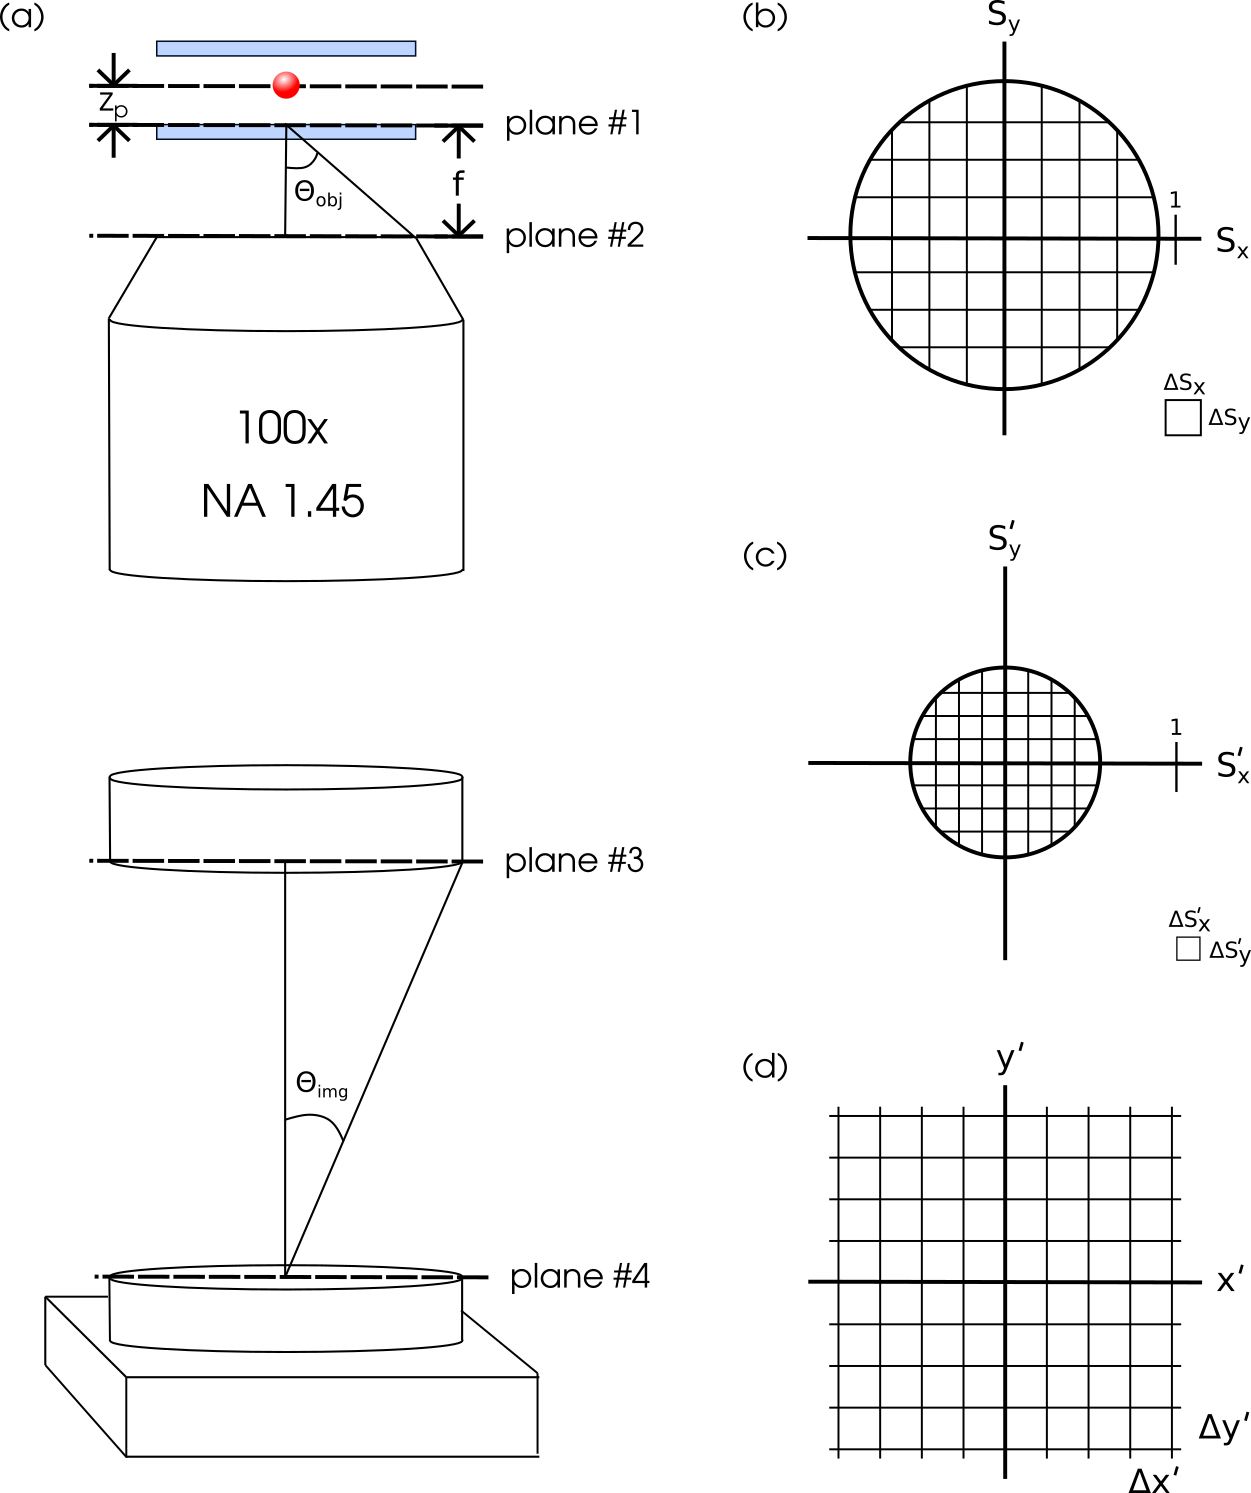
\includegraphics[width=0.95\textwidth]{debyewolf_schematic}
  \caption{Diagram depicting the planes at which the fields are evaluated.
    (a) The fields propagate through the focal plane (plane \#1) of the objective,
    are collected by the objective's entrance pupil (plane \#2), focused by the tube lens (plane 3)
    and arrive at the imaging plane (plane \#4) of the camera. (b) and (c) illustrate the
    discretization of the electric field strength factor at plane \#2 and \#3 respectively.
    (d) illustrates the discretization of the electric field at the imaging plane, plane \#4.}
  \label{fig:debye_schematic}
\end{figure}

\section{Modeling the optical train}

With the exception of a coherent illumination source, our holographic microscope
can be reduced to the four essential components of a conventional microscope:
the sample, an objective, a tube lens, and a camera. In the previous chapter,
we described the scattering of a plane wave by a spherical scatterer up to
the focal plane of the objective. We will now evaluate the scattered field and
the plane wave at several interfaces as they propagate along the optical axis
to the camera plane. Figure \ref{fig:debye_schematic}(a) illustrates the four planes
of interest. In the following sections, we will perform the following calculations
for the scattered field:
\begin{enumerate}
\item Evaluate the electric field strength factor for the scattered field at
  the entrance pupil of the objective, plane \#\num{2}.
\item Account for the axial displacement of the particle away from the focal
  plane of the objective.
\item Compute the electric field strength factor at the exit of the tube lens, plane \#3,
  by accounting for the angular demagnification imposed by the objective.
\item Use a near-field-to-far-field transform to determine the scattered
  fields at the imaging plane of the camera, plane \#4.
\end{enumerate}
Figure \ref{fig:debye_schematic}(b) presents the geometries used to define the
fields at the entrance pupil of the objective, at the tube lens, and at the camera's
imaging plane, planes \#\num{2}, \#\num{3}, and \#\num{4}, respectively.
The linearity of our optical system allows us to consider the incident field
and scattered field separately. We will derive the transformations for the
scattered field first and then summarize the corresponding transformation for the
plane wave.

\subsection{Scattering to the entrance pupil}

In \autoref{ch:hvm}, we computed the fields resulting from the scattering of
a plane wave by a homogeneous sphere embedded in an otherwise
homogeneous medium. As depicted in Fig.~\ref{fig:debye_schematic}(a), we
propagate the radially expanding scattered fields through the focal plane (plane \num{1} in
Fig.~\ref{fig:debye_schematic}) and onward to the objective's entrance pupil a distance
$z_p + f$ below the particle, where $f$ is the focal length of the objective.
\begin{figure}
  \centering
  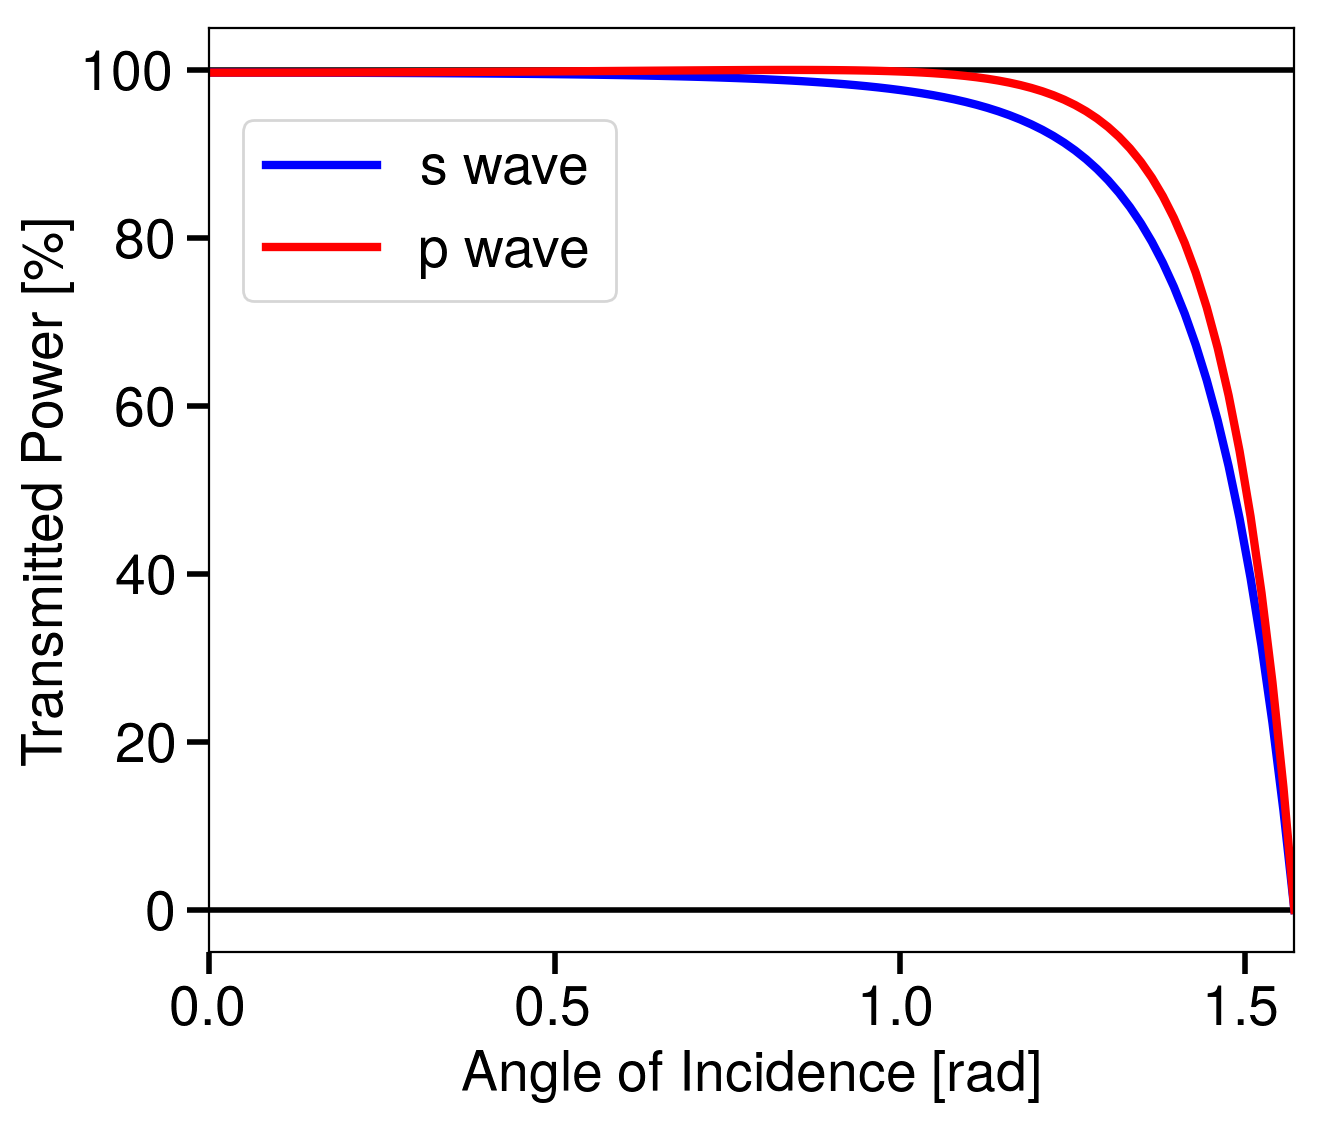
\includegraphics[width=0.73\textwidth]{waterglass}
  \caption{The Fresnel transmission coefficients for $s-$ and $p$-polarized
  waves refracting through a water-glass interface.}
  \label{fig:waterglass}
\end{figure}

During this transit, the fields reflect and refract at the water-glass interface as they
exit the sample volume. Fig.~\ref{fig:waterglass} presents the Fresnel transmission
coefficients for rays incident on the interface at angle $\theta$.
Because the scattered fields we record are dominated by low-angle scattering,
we safely neglect the reflection and refraction at this interface. Furthermore,
because we utilize an
oil-immersion objective whose refractive index, $n_{\text{oil}}$,
nearly matches that of glass, we also neglect the secondary refraction at the
glass-oil interface treated by Ovryn and Izen \cite{izen00}.

Our objective  (Nikon Plan Apo, $\num{100}\times$, numerical aperture $\num{1.45}$,
oil immersion) was manufactured to have a parfocal length of $\SI{135}{\um}$.
At this distance, wavelength, and particle size, the scattered field is in the far-zone,
also known as the Fraunhofer zone, given by $z_p + f >> a_p^2/\lambda$. In this
regime, the wave's radial dependence can be factored out from its angular dependence,
\begin{equation}
  \label{eq:strength_factor}
  \vec{E}_s(r, \theta, \phi) \approx  \vec{E}_s(\theta, \phi) \frac{e^{ikr}}{r}.
\end{equation}
The term $\vec{E}_s(\theta, \phi)$ is known as the strength factor and
depends only on the polar angle $\theta$ and the azimuthal angle $\phi$.
For computational ease, we parameterize the strength factor as $\vec{E}_s(s_x, s_y)$
with the direction cosines $s_x=\cos{\phi}\sin{\theta}$ and $s_y = \sin{\phi}\cos{\theta}$.

Casting the scattered field in terms of its strength factor will simplify
several of the upcoming calculations. Equation~\eqref{eq:strength_factor} however
is only valid when the scattered field is in the far-field regime.
Ovyrn and Izen\cite{izen00} estimate that adopting this approximation induces a maximum
$\SI{2}{\percent}$ error in the calculated intensity in the range of particle
sizes and locations that we consider here.
%% FIXME: Check this claim and possible add a reference
% to an appendix that justifies these claims.

\begin{figure}
  \centering
  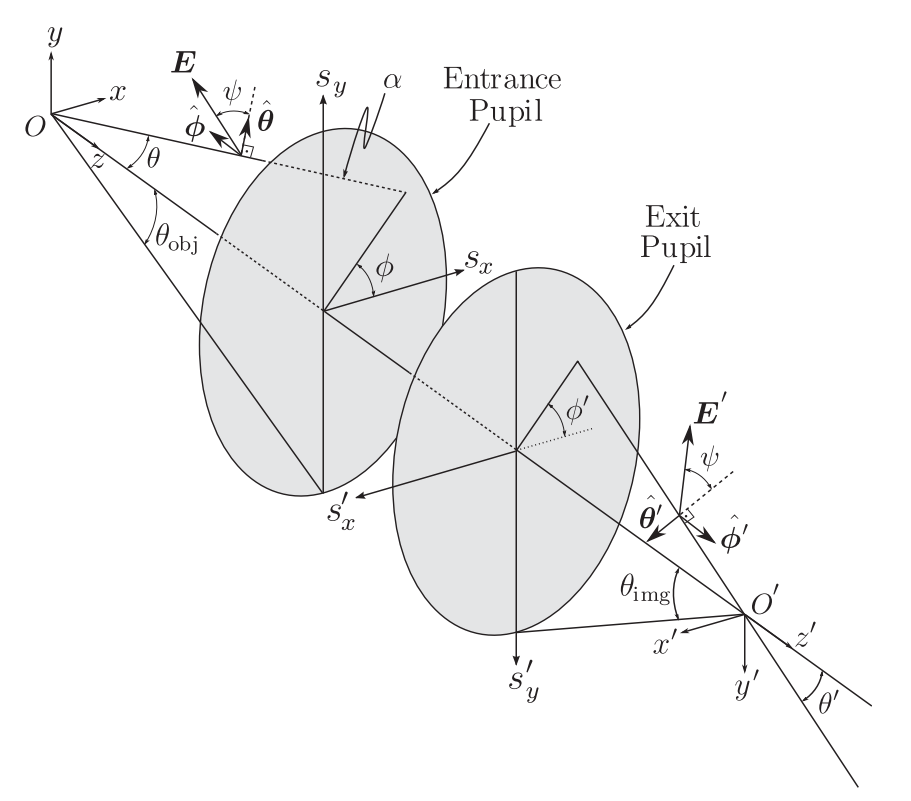
\includegraphics[width=0.75\textwidth]{debye_geom}
  \caption{The two spherical geometries necessary for our description. The un-primed coordinates
    describe the spherical geometry for waves entering the entrance pupil; the primed coordinates
    describe the spherical geometry for waves exiting the tube lens. $\theta_{\text{obj}}$ and
    $\theta_{\text{img}}$ maximal half-angle of the cone of light that can enter or exit
    the objective lens and tube lens, respectively (Ref. \cite{capoglu12}, Fig. 13).}
  \label{fig:debye_geom}
\end{figure}

\subsection{ Displacement of the scattered field}

The electric field strength factor, $\vec{E}(\theta, \phi)$, is independent
of distance and will be assumed to be originating from
the origin of the focal plane in the near-field-to-far-field transform rather
than the particle's location a distance $z_p$ above.
Following Goodman\cite{goodman05}, we account for the scatterer's displacement
along the optical axis with a relative phase shift\footnote{The sign convention used here is appropriate for a scattered positioned a distance $z_p$ in the $-\uvec{z}$ direction.}.
\begin{equation}
  \label{eq:entrance_pupil}
    \vec{E}_s(\theta, \phi)|_{\text{scatterer plane}} \approx \vec{E}_s(\theta, \phi)|_{\text{focal plane}} e^{-i\frac{2\pi}{\lambda}z_p\cos{\theta} }.
  \end{equation}

\subsection{Collection}
In its transit through the optical train from plane \#2 to the camera plane \#3, 
the scattered field experiences an angular demagnification 
that imparts a scaling, polarization rotation, and lensing effect.
The overall effect can be accounted for by
a coordinate transformation governed by the Abbe sine condition and by scaling
each ray to obey the conservation of energy.

The Abbe sine condition,
\begin{equation}
  M = \frac{n_m \sin \, \theta}{n^{\prime} \sin \, \theta^{\prime}}
  \label{eq:abbe_sine}
\end{equation}
is necessary for sharp imaging \cite{capoglu12} and is rigorously
satisfied in modern optical designs.
Here, $M$ is the system's lateral magnification, $n_m$ is the medium's refractive index,
and $n'\approx 1$ is the refractive index at the camera plane.
A ray entering the objective lens at angle $\theta$ relative to the optical axis exits
the tube lens at an angle $\theta^{\prime}$ with a polarization rotation of
$\SI{180}{\degree}$ as portrayed in Fig.~\ref{fig:debye_geom}.
Additionally, angular demagnification concentrates the electromagnetic radiation
to a smaller solid angle and increases the magnitude of the electric field strength
factor. Accounting for these three effects, we relate the electric field strength at the
entrance pupil of the objective to the electric field strength at the tube lens as
  \begin{equation}
    \begin{split}
    \vec{E}_s'(\theta', \phi')\cdot\hat{\theta'} & = - M \sqrt{ \frac{n'\cos{\theta'}}{n\cos{\theta}}}\vec{E}_s(\theta, \phi)\cdot\hat{\theta} \hspace{0.2 in}\text{and}\\
    \vec{E}_s'(\theta', \phi')\cdot\hat{\phi'} & = - M \sqrt{ \frac{n'\cos{\theta'}}{n\cos{\theta}}}\vec{E}_s(\theta, \phi)\cdot\hat{\phi}.
    \end{split}
  \end{equation}

For computational ease, we again adopt direction cosines $s'_x = \cos \, \phi'\sin \, \theta'$ and
$s'_y=\sin{\phi'}\sin{\theta'}$ such that the electric field strength
factor exiting the tube lens is parameterized as $\vec{E}_s^{\prime}(s'_x, s'_y)$. Under this
coordinate transformation, the Abbe sine condition given by Eq.~\eqref{eq:abbe_sine} can
readily be seen as a linear scaling of the magnitudes of the direction cosines

\begin{equation}
  M = \frac{n_m \sqrt{s_x^2 + s_y^2 }}{n^{\prime} \sqrt{s_x^{\prime 2} + s_y^{\prime 2} }}.
\end{equation}
  
\subsection{Refocusing the fields to the camera plane}
Finally we utilize a near-field-to-far-field transform to propagate the scattered
field from the tube lens to the imaging plane.
The Debye-Wolf diffraction integral transforms the electric field strength factor at a lens
surface to the scattered field, $\vec{E}_{s,\text{img}}$, present in the focal plane of that
lens:
\begin{equation}
  \vec{E}_{s,\text{img}}(x', y') = \frac{i k'}{2 \pi} \iint_{\Omega_{\text{img}}} \vec{E}_s'(s'_x, s'_y) \frac{e^{-ik'(s'_xx'+s'_yy')}}{\cos{\theta'}}ds'_xds'_y 
  \label{eq:debyewolf}
\end{equation}
where $k'$ is the wavenumber in the medium above the camera and $\Omega_{\text{img}}$
is the domain of integration set by the Abbe sine condition and the condition
that $s_x^2+s_y^2 \le \text{NA}/n_{\text{oil}}$. Note that $\cos \, \theta' = \sqrt{ 1 - (s_x^{\prime 2} + s_y^{\prime 2} )}$. Several points are worth mentioning:
\begin{enumerate}
\item This integral acts as an inverse of Huygen's principle; a spherical wave is
  decomposed into a multitude of plane waves whose phase relations and subsequent
  interference produce the same effect as the original spherical wave.
\item The Debye-Wolf transformation takes $\vec{E}'_s$, a strength factor with units
  $\si{\volt\meter}$, defined in spherical coordinates on plane \#\num{3} and
  returns the electric field in Cartesian coordinates in plane \#\num{4}.
\item The transformation appears to be distance agnostic; the distance
  between plane \#\num{3} and \#\num{4} never explicitly appears. However the domain
  of integration, $\Omega_{\text{img}}$, is limited by the Abbe sine condition
  such that the planes \#\num{3} and plane \#\num{4} must be separated by $M \, f$.
\end{enumerate}

The Debye-Wolf integral can account for phase aberrations
due to imperfections in the optical train with an aberration function, $\Phi(s'_x,s'_y)$,
which measures the deviation of the wavefront from a perfect spherical shape \cite{wolf1959}.
To do so, the integrand of the Debye-Wolf integral is multiplied by a phase term
$e^{ik'\Phi(s'_x,s'_y)}$. We will not consider aberrations, however, because
the goal of this study is to access limitations in hologram formation
under ideal conditions.

With the exception of the $k'$ in the phase term and the $\cos{\theta'}$ 
modifying the differential element, we should recognize the
Debye-Wolf integral as a Fourier transform. We will discretize this
Fourier transform subject to sampling and aliasing conditions described
in the appendix \ref{app:discretize_dw}. Here we summarize and interpret the result:
\begin{equation}
  \begin{split}
    \vec{E}_{s,\text{img}}( m \Delta_x, n \Delta_y) & \approx \frac{i k' \Delta s'_x \Delta s'_y}{2 \pi} e^{-i2\pi \left ( \frac{s'_{x_o}}{\Delta s'_x N_p} m + \frac{s'_{y_o}}{\Delta s'_yN_q} n \right ) } \vec{E}_s'\left [ m, n \right ] \\
    \vec{E}_s'\left [ m,n \right ] & = \sum_{p=0}^{N_p-1}\sum_{q=0}^{N_p-1}\vec{G}'\left [p,q\right ] e^{-i2\pi \left ( \frac{pm}{N_p}+\frac{qn}{N_q} \right ) } \\
    \vec{G}'(s'_x,s'_y) & \doteq \vec{E}'_s(s'_x,s'_y)\frac{\vec{E}'_s(s'_x,s'_y)}{\cos{\theta'}}e^{-ik'\Phi(s'_x,s'_y)}
  \end{split}
  \label{eq:complete_dw}
\end{equation}
where the the $s_x'$-$s_y'$ plane is discretized into a
$N_p$ by $N_q$ grid with a sampling period $\Delta s_x'$ along the $s_x'$ axis and
$\Delta s_y'$ along the $s_y'$ axis, and the $x'$-$y'$ plane is similarly discretized with
sampling periods $\Delta x = 2\pi \, / \, k' \Delta s_x' N_p$ and $\Delta y = 2\pi \, / \, k' \Delta s_y' N_p$.
Note that the vector functions with parens encasing their arguments represent
continuous functions whereas those with square brackets encasing their arguments represent
discrete approximations of continuous functions.

The Debye-Wolf integrand rapidly oscillates with respect to its arguments $s_x'$ and $s_y'$.
To ensure our approximation to the integral \eqref{eq:debyewolf} converges, we
must appropriately sample the $s_x'$-$s_y'$ grid. In addition, we must mitigate any
aliasing that may result from the Fourier transform in Eq.~\eqref{eq:complete_dw}.
Further restricting our discretization scheme, the sampling periods $\Delta_x$
and $\Delta_y$ should be comparable to the size of a pixel. These competing constraints
can be cast as an integer equation and approximately solved as demonstrated
in appendix \ref{app:discretize_dw}.

\subsection{Superposition of the propagated fields}

The propagation of the incident plane wave through the optical system is more easily explained.
The incident field travels parallel to the optical
axis towards the entrance pupil of the objective. The objective
and tube lens then laterally magnify the incident field and induce a
$\SI{180}{\degree}$-shift in phase.
The incident field maintains its polarization and arrives at the imaging plane as
\begin{equation}
  \vec{E}'_{\text{inc}}(x',y') = -\frac{1}{M}\sqrt{\frac{n_1}{n_2}} \vec{E}_{\text{inc}}(x,y).
\end{equation}
The image in the camera plane is then
\begin{equation}
  I(x', y') = \preint \left | \vec{E}'_{\text{inc}}(x',y') + \vec{E}'_s(x', y') \right |^2.
\end{equation}
  
\section{Comparison to Scalar Diffraction Theory}

Having accounted for the propagation of the incident field and the scattered
field through the optical system, we are now ready to assess differences
between the vector theory and the scalar theory. As shown in Fig.~\ref{fig:debye_difference_ps},
the two theories produce nearly identical holograms for a \SI{1.0}{\um} diameter
polystyrene particle with refractive index $n_{\text{p}}=1.59$ displaced
\SI{13.5}{\um} above the focal plane; the difference in intensity at each
pixel in the respective holograms is well below the sensitivity of our camera.

\begin{figure}
  \centering
  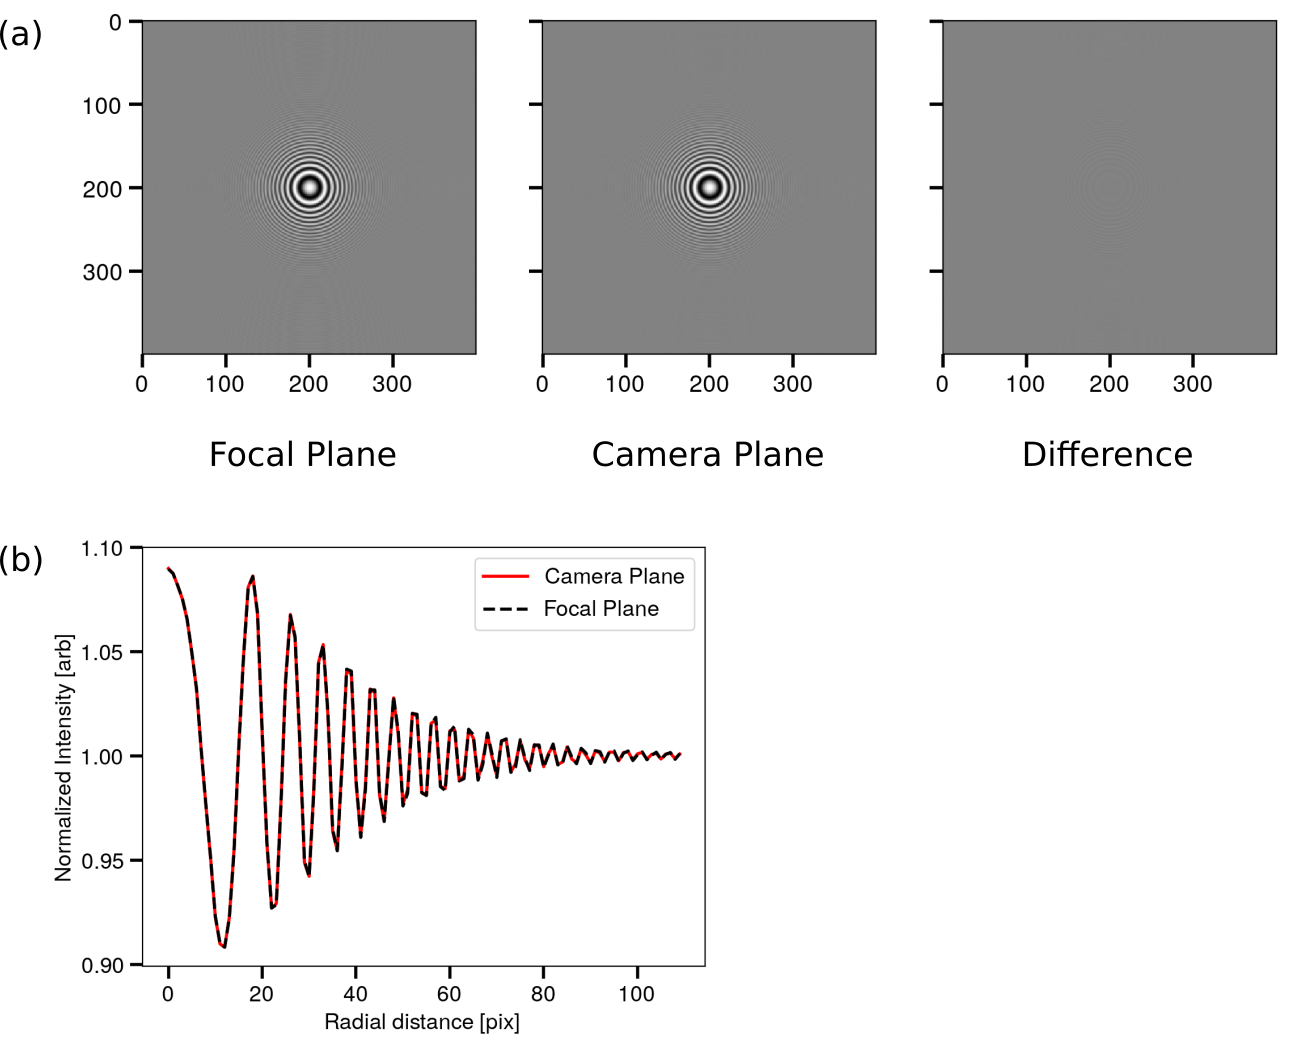
\includegraphics[width=\textwidth]{debyewolf_differences}
  \caption{(a) Holographic images produced in the focal plane of the objective lens and
    the imaging plane of the camera, and an image of their difference.
    (b) Radial profiles of holographic snapshots taken
    in the focal plane of the objective and the imaging plane of the camera.
    These particular holographic features were produced by a $\SI{1.0}{\um}$
    diameter polystyrene particle $\SI{13.5}{\um}$ above the focal plane.}
  \label{fig:debye_difference_ps}
\end{figure}

To systematically assess the differences between the two theories,
we use Eq.\eqref{debyewolf} to synthesize holographic
images as they would appear in the camera plane. Synthetic holograms
were computed for spheres with radii ranging from
$a_{\text{p}}=\SI{0.5}{\um}$ to $\SI{5}{\um}$, refractive indexes from
$n_{\text{p}}= \SI{1.4}{}$ to $\SI{1.8}{}$, and displacements from the focal plane,
$z_{\text{p}}=\SI{5}{\um}$ to $\SI{50}{\um}$.
We then fit each synthetic hologram to the scalar theory representing
images in the focal plane of the objective lens as described
in \autoref{ch:hvm}. The degree to which the resulting fit parameters differ
from the known scatterer properties set a lower bound for the error of adopting
the scalar theory in favor of the vector theory.

Over the majority of parameter space, the error in diameter and
axial displacement are bounded by $\SI{1}{\nm}$ while the error
in refractive index is bounded by $\SI{0.001}{}$; in all three
parameters, the maximum error is less than the reported resolution of
the technique \cite{krishnatreya14}. In certain regions of parameter
space, our discretization scheme could not adequately sample the
highly-oscillatory integrand in Eq.~\eqref{eq:debyewolf}.
No synthetic holograms are available in this range.

\section{Discussion}

This chapter provides a detailed treatment of the scattered field
and incident field as they propagate through the optical train to the camera
to produce an image.
We determined that accounting for
the effects of refraction, reflection, lateral magnification, and angular
demagnification does not change the resulting hologram by a measurable amount.
The existing formulation therefore is optimal in this sense. This optimality
was not established before this study. Additionally
the computational complexity of producing
the image in the camera plane greatly exceeds that of producing the
image in the focal plane; for this reason, we recommend the use of the
scalar theory in fitting experimental holograms with ideal optics.
For real lenses, some degree of phase-aberrations are imparted by
the optical train; in the case of non-ideal holographic imaging,
our theory provides a model which accounts for phase-aberrations,
including spherical aberrations.
